%%%%%%%%%%%%%%%%%%%%%%%%%%%%%%%%%%%%%%%%%%%%%%%%%%%%%%%%%%%%%%%%%%%%%%
% LaTeX Template: Beamer arrows
%
% Source: http://www.texample.net/
% Feel free to distribute this template, but please keep the
% referal to TeXample.net.
% Date: Nov 2006
% 
%%%%%%%%%%%%%%%%%%%%%%%%%%%%%%%%%%%%%%%%%%%%%%%%%%%%%%%%%%%%%%%%%%%%%%
% How to use writeLaTeX: 
%
% You edit the source code here on the left, and the preview on the
% right shows you the result within a few seconds.
%
% Bookmark this page and share the URL with your co-authors. They can
% edit at the same time!
%
% You can upload figures, bibliographies, custom classes and
% styles using the files menu.
%
% If you're new to LaTeX, the wikibook is a great place to start:
% http://en.wikibooks.org/wiki/LaTeX
%
%%%%%%%%%%%%%%%%%%%%%%%%%%%%%%%%%%%%%%%%%%%%%%%%%%%%%%%%%%%%%%%%%%%%%%

\documentclass[9pt]{beamer} %
\usetheme{CambridgeUS}
\usepackage[utf8]{inputenc}
\usepackage[spanish]{babel}
\usefonttheme{professionalfonts}
\usepackage{times}
\usepackage{tikz}
\usepackage{amsmath}
\usepackage{verbatim}
\usetikzlibrary{arrows,shapes}
\usepackage{framed, color}
\definecolor{shadecolor}{rgb}{0.690, 0.933, 0.525}


\author[Universidad de Granada]{Daniel López García\\ Lothar Soto Palma\\\textit{Universidad de Granada}}
\title{Ingeniería de sistemas de información\\ Búsquedas en Intenet}

\begin{document}

% For every picture that defines or uses external nodes, you'll have to
% apply the 'remember picture' style. To avoid some typing, we'll apply
% the style to all pictures.
\tikzstyle{every picture}+=[remember picture]

% By default all math in TikZ nodes are set in inline mode. Change this to
% displaystyle so that we don't get small fractions.
\everymath{\displaystyle}

\begin{frame}
\titlepage
\end{frame}

\begin{frame}
\frametitle{Índice}
\tableofcontents
\end{frame}
\begin{frame}
	\frametitle{Introducción}
	Internet se ha convertido en una fuente de conocimiento masiva, como consecuencia los motores de búsqueda web se han vuelto muy importantes y la necesidad de obtener una arquitectura para estos sistemas que óptimice la realización de búsquedas es ahora una necesidad.
	
	\medskip
	En la web nos encontramos con varios problemas para realizar búsquedas:
		\begin{itemize}
			\item Escalabilidad
			\item Volatilidad 
			\item Variabilidad
		\end{itemize}
\end{frame}
\begin{frame}
	\frametitle{Arquitectura de un buscador.}
Los motores de búsqueda que operan en Internet tienen comúnmente una arquitectura centralizada, los elementos que componen esta arquitectura son:
		\begin{figure}[H]
			\centering
			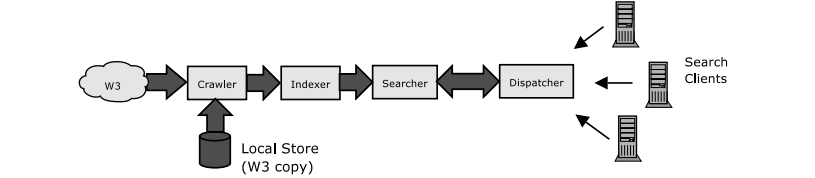
\includegraphics[scale=0.6]{./img/modeloreferente.png}
		\end{figure}
		\begin{itemize}
			\item \textbf{Crawler}: Se encarga de la agregación al sistema de los documentos que posteriormente serán indexados para su búsqueda.
			\item \textbf{Indexer}: El indexador es el módulo que se encarga construir una estructura de acceso rápido llamada índice.
			Existen diversos modelos de indexación algunos de ellos son:
			\begin{itemize}
				\item Modelo binario.
				\item Modelo Vectorial.
				\item Modelo Probabilistico.
			\end{itemize}
		
		\end{itemize}
\end{frame}

\begin{frame}
	\frametitle{Arquitectura de un buscador.}

	\begin{itemize}
		\item \textbf{Searcher}: El buscador es aquel módulo que se encarga realizar las consultas sobre el índice.
		\item \textbf{Dispatcher}: Es el encargado de la recepción de la consulta realizada desde el buscador y enviarla al Searcher para posteriormente obtener una lista ordenada en función de una puntuación denominada relevancia. Algunos métodos para calcular la relevancia son:
		\begin{itemize}
			\item Coeficiente de Jaccard en modelos de indexación binarios.
			\item Coseno en modelos de indexación vectorial de tipo tf-idf.
		\end{itemize}
		
	
	\end{itemize}
\end{frame}
\begin{frame}
	\frametitle{Arquitectura de Google}
	\begin{figure}
	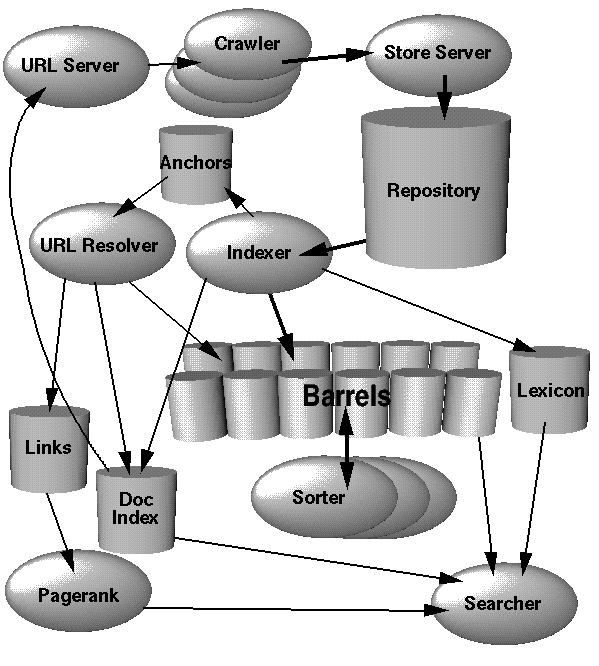
\includegraphics[scale=0.33]{img/google_architecture.png}
\end{figure}
	\end{frame}
\begin{frame}
	\frametitle{}
\begin{itemize}
	\item Las estructuras de datos usadas están optimizadas para manejar grandes colecciones de datos.
	\item Se hace uso del modelo MapReduce para la creación de los índices.
	\item El crawling se realiza usando una gran cantidad de crawlers de forma distribuida.
	\item Las páginas webs obtenidas mediante el crawling se almacenan comprimidas en un repositorio. La función de indexación descomprime los documentos y los parsea para crear el indice.
	\item Otro aspecto a tener en cuenta es el texto de los enlaces, ya que normalmente contienen la mejor descripción de la página.
\end{itemize}		
\end{frame}

\begin{frame}
	\frametitle{PageRank}
Proporciona una medida de la importancia de la página en función de las páginas que contienen enlaces a la misma. Este valor se calcula sumando el número de enlaces a la pagina normalizados por un parámetro $d$ que indica la importancia de la página de la que procede el enlace.

\[
PR(A)=(1-d)+d(\frac{PR(T_1)}{C(T_1)}+...+\frac{PR(T_n)}{C(T_n)})
\]
\end{frame}
\begin{frame}
	\frametitle{Enlaces de referencia.}
	\begin{thebibliography}{9}
		
		\bibitem{Multi-tier architecture for Web Search Engines}
		\url{http://www.cwr.cl/la-web/2003/stamped/15_risvik_k-updates.pdf}
		\bibitem{The anatomy of a large-scale hypertextual Web search engineThe anatomy of a large-scale hypertextual Web search engine}
		\url{http://www.sciencedirect.com/science/article/pii/S016975529800110X?via\%3Dihub}
		
	\end{thebibliography}
\end{frame}
\end{document}
              
            